\section{Quality assurance}

Verification focuses on internal characteristics, ensuring that the software is built correctly, while validation concerns external characteristics, ensuring that the right software is being built.
\begin{definition}[\textit{Quality assurance }]
    Quality assurance establishes policies and processes to have quality in software development.
\end{definition}
Quality encompasses various aspects:
\begin{itemize}
    \item Elimination of defects or bugs.
    \item Resolution of issues hindering the fulfillment of non-functional requirements or causing degradation of software qualities.
    \item External qualities such as performance and availability.
    \item Internal qualities like maintainability.
\end{itemize}
\begin{definition}[\textit{Failure}]
    Failure is the termination of a product's ability to perform a required function or its incapacity to operate within predefined limits. 
    It is an event where a system or its component fails to fulfill a specified function.
\end{definition}
\begin{definition}[\textit{Fault}]
    A fault is the observable manifestation of a defect.
\end{definition}
\begin{definition}[\textit{Defect}]
    A defect is an imperfection or deficiency in a program.
\end{definition}
\begin{definition}[\textit{Error}]
    An error results from a human action introducing an incorrect result.
\end{definition}
\begin{figure}[H]
    \centering
    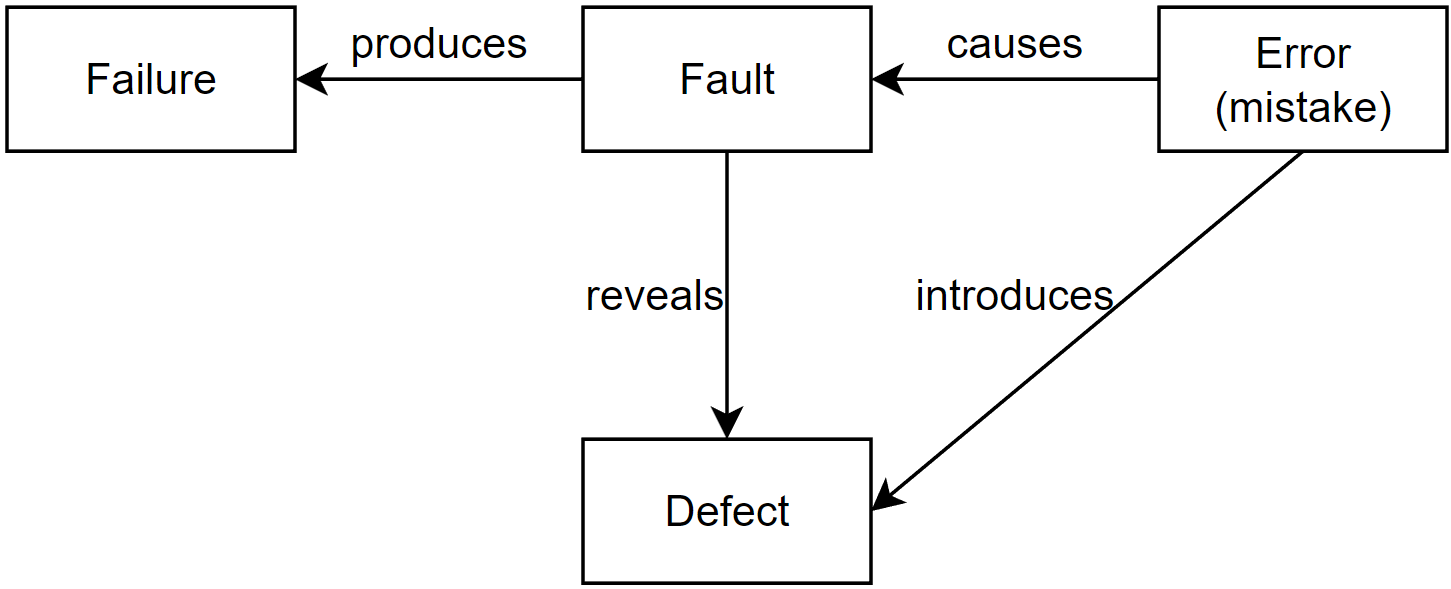
\includegraphics[width=0.6\linewidth]{images/ver.png}
    \caption{Failure, fault, defect, and errors}
\end{figure}
Achieving zero-defect software is practically impossible, necessitating careful and continuous quality assurance. 
Ideally, every artifact should undergo quality assurance, including verification artifacts, which must themselves be verified.

\paragraph*{Structural engineering and software engineering}
In structural engineering, when tasked with constructing a bridge intended to support heavy trucks (40 tons), a straightforward approach involves subjecting the bridge to a load test with, for instance, 50 tons. 
Remarkably, this single test scenario effectively covers a spectrum of potential cases. \\
On the contrary, in software engineering, where the goal is to develop a program, the absence of continuous behavior complicates the verification process. 
Testing a program with a single data point provides limited insights into its performance at other points.
Consequently, the choice of verification techniques varies depending on the level of implementation, as illustrated below:
\begin{figure}[H]
    \centering
    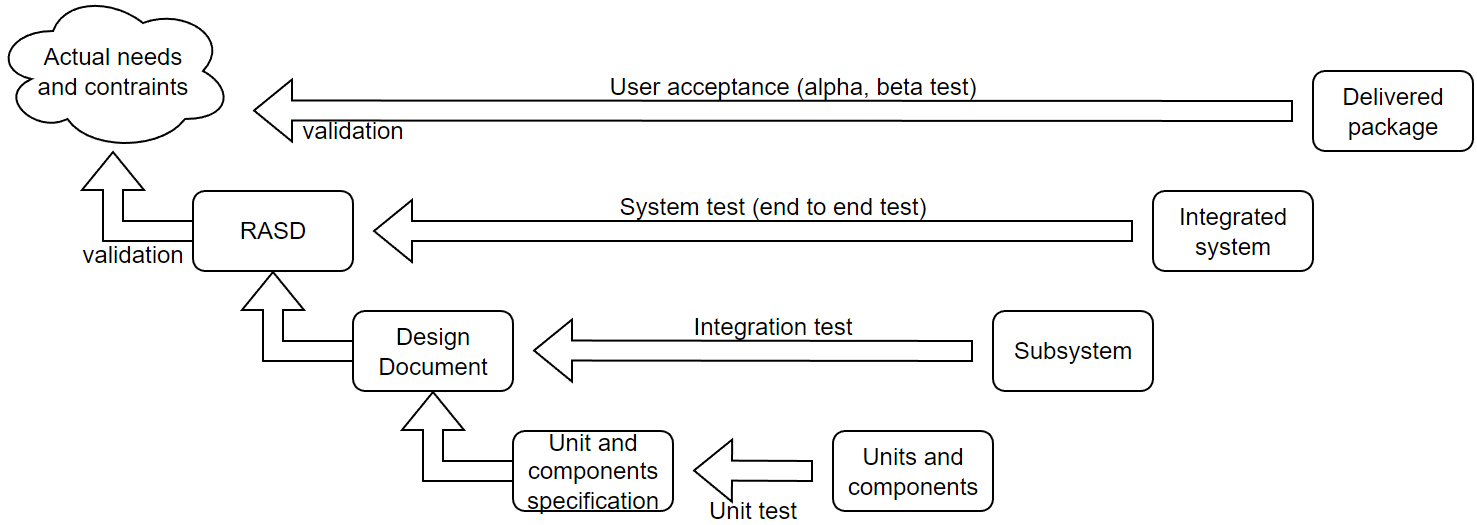
\includegraphics[width=1\linewidth]{images/ver1.png}
\end{figure}

\paragraph*{Possible approaches}
There are two primary approaches for testing a program:
\begin{itemize}
    \item \textit{Static analysis}: this analysis occurs directly on the program's source code without execution. 
        It's important to note that the properties examined are dynamic.
    \item \textit{Dynamic analysis}: also known as testing, dynamic analysis involves executing the program's sources, typically through sampling. 
        During this analysis, the actual behavior of the program is assessed in comparison to the expected behavior.
\end{itemize}
\begin{table}[H]
    \centering
    \begin{tabular}{cc}
    \hline
    \textbf{Static analysis}          & \textbf{Dynamic analysis}    \\ \hline
    At compile time                   & At runtime                   \\
    Related to source code            & Related to software behavior \\
    Without execution of the software & While executing the software \\
    On generic (or symbolic) inputs   & On specific inputs           \\ \hline
    \end{tabular}
\end{table}